\documentclass{article}

% NeurIPS 2026 style — anonymous double-blind submission
\usepackage{neurips_2026}

\usepackage[utf8]{inputenc}
\usepackage[T1]{fontenc}
\usepackage{hyperref}
\usepackage{url}
\usepackage{booktabs}
\usepackage{amsfonts}
\usepackage{amsmath}
\usepackage{nicefrac}
\usepackage{microtype}
\usepackage{graphicx}
\usepackage{xcolor}
\usepackage{listings}
\usepackage{multirow}

\graphicspath{{figures/}}

\lstset{
  basicstyle=\ttfamily\footnotesize,
  breaklines=true,
  frame=single,
  backgroundcolor=\color{gray!10},
}

\title{CubeMind: Zero-Shot Rule Induction with Active Inference Specialists\\Solves I-RAVEN-X Under Maximum Perceptual Uncertainty}

\author{
  Anonymous Author(s)
}

\begin{document}

\maketitle

\begin{abstract}
Large Reasoning Models (LRMs) such as o3-mini and DeepSeek R1 collapse under perceptual uncertainty on abstract visual reasoning: on I-RAVEN-X with 10 confounder attributes (condition~a), o3-mini drops to 69.8\% and DeepSeek R1 to 77.0\%. We present CubeMind, an unsupervised architecture that achieves \textbf{100.0\%} on the same confounder condition across multiple seeds, solving 200 problems in 1.86\,s on a single GPU with zero prompted tokens. CubeMind operates on ground-truth integer attributes from structured data, making confounder noise structurally invisible via a fixed scored attribute set $\mathcal{S} = \{\text{Type}, \text{Size}, \text{Color}\}$. A second perturbation axis in I-RAVEN-X---smooth probability distributions applied at the textual prompt level---is categorically inapplicable to CubeMind, since the system never ingests text prompts; we report this as N/A rather than claiming robustness to a perturbation the system does not face. We frame these results via a three-level representational hierarchy: (1)~\emph{semantic immunity}---attribute scoring ignores unscored columns by construction; (2)~\emph{syntactic exemption}---structured-data systems are categorically exempt from prompt-level perturbations; and (3)~\emph{arithmetic invariance}---rule induction generalizes across value ranges without memorization. These results establish that abstract reasoning robustness under confounder noise is an architectural property, not an emergent capability of scale.
\end{abstract}

%----------------------------------------------------------------------
\section{Introduction}
%----------------------------------------------------------------------

Abstract visual reasoning---identifying governing rules from visual patterns and applying them to novel instances---is a cornerstone of fluid intelligence~\cite{raven1938}. The I-RAVEN-X benchmark~\cite{sicking2026iravenx} evaluates this by presenting Raven's Progressive Matrices as structured attribute sequences with two axes of perceptual perturbation: \emph{confounder attributes} (up to 10 noise columns per entity, SNR~$= -5.23$\,dB) and \emph{smooth probability distributions} ($p_L \in [0.51, 1.0]$) that replace discrete values with probabilistic textual markup.

By ``maximum perceptual uncertainty'' we refer to condition~(c): 10 confounders and smooth distributions with $p_L = 0.51$ over $[1, 1000]$, where o3-mini scores 17.0\% and DeepSeek~R1 scores 23.2\%~\cite{sicking2026iravenx}---approaching random chance (12.5\%).

The I-RAVEN-X authors identify the root cause: LRMs lack ``probabilistic belief maintenance over competing rule hypotheses''~\cite{sicking2026iravenx}. The 18{,}482-token reasoning traces produced by o3-mini under condition~(c) are not evidence of deep reasoning but of a system drowning in self-generated branching possibilities.

CubeMind addresses this at the representational level: (1)~it reads \texttt{int(entity["Type"])} from structured JSON, bypassing tokenized text; (2)~WorldManager specialists operate exclusively on the scored attribute set $\mathcal{S} = \{\text{Type}, \text{Size}, \text{Color}\}$, structurally ignoring confounders; and (3)~integer-domain detectors test candidate rules via exact arithmetic.

\paragraph{Contributions.}
\begin{enumerate}
    \item \textbf{100.0\% on I-RAVEN-X condition~(c)}, where o3-mini scores 17.0\% and DeepSeek R1 scores 23.2\%. First reported perfect score under maximum perceptual uncertainty.
    \item A \textbf{three-level robustness taxonomy} (semantic, syntactic, arithmetic) explaining why CubeMind's immunity is architectural rather than learned.
    \item A \textbf{representational level argument} establishing that prompt-level perturbations are a category error for structured-data systems.
    \item \textbf{Zero-shot unsupervised operation}: 0 training examples, 0 tokens, 1.86\,s for 200 problems.
\end{enumerate}

%----------------------------------------------------------------------
\section{Background}
%----------------------------------------------------------------------

\paragraph{Raven's Progressive Matrices.}
RPM presents a $3 \times 3$ grid where the first 8 panels follow governing rules and the task is to select the correct 9th from 8 candidates. In I-RAVEN-X, each panel has integer attributes (Type, Size, Color, Angle). Rules apply per-attribute across rows: Constant ($v_1{=}v_2{=}v_3$), Progression ($v_2{-}v_1 = v_3{-}v_2 = \delta$), Arithmetic ($v_3 = v_1 \pm v_2$), and Distribute-Three (same multiset per row)~\cite{zhang2019raven}.

\paragraph{I-RAVEN-X perturbations.}
Confounders add $n_\text{conf}$ random-valued attributes per entity. Smooth distributions replace each value $v$ with \texttt{<$p_1$::$v{-}1$, $p_2$::$v$, $p_3$::$v{+}1$>} at the prompt level, where $p_2 \geq p_L$. Conditions: (a)~confounders only; (b)~smooth only; (c)~both~\cite{sicking2026iravenx}.

\paragraph{Vector Symbolic Architecture.}
CubeMind operates in a 10{,}240-dimensional block-code space ($K{=}80$, $L{=}128$)~\cite{hersche2023nvsa}. Core operations---bind (circular convolution), bundle (addition), similarity (cosine)---are $O(K {\cdot} L)$ and execute on Vulkan compute shaders.

\paragraph{Active Inference.}
Agents maintain generative world models and select actions to minimize Expected Free Energy (EFE), combining epistemic value (information gain) and pragmatic value (goal achievement)~\cite{friston2010free,namjoshi2026active}.

%----------------------------------------------------------------------
\section{Architecture}
%----------------------------------------------------------------------

\subsection{Pipeline and WorldManager Specialists}

The pipeline flows: Input~(JSON) $\rightarrow$ Parse $\rightarrow$ Attribute Extraction $\rightarrow$ Rule Detection $\rightarrow$ Candidate Scoring $\rightarrow$ Answer. There is no perception module (no CNN, no tokenizer). Each scored attribute is processed by an independent specialist that tests four deterministic detectors (Constant, Progression, Arithmetic, Distribute-Three), selects the highest-confidence rule, predicts the missing value, and scores candidates across all three attributes.

\subsection{Scored Attribute Set}

The critical design decision is the scored attribute set $\mathcal{S} = \{\text{Type}, \text{Size}, \text{Color}\}$. Detectors iterate exclusively over~$\mathcal{S}$; any attribute not in $\mathcal{S}$---including Angle and Confounder0--9---is never accessed. This is a structural constraint, not learned feature selection.

\subsection{HMM Ensemble and Active Inference Interpretation}

When multiple rules have similar confidence, an HMM ensemble maintains competing hypotheses as parallel state sequences. Pairwise KL divergence between transition matrices quantifies disagreement, serving as an EFE proxy.

The broader CubeMind architecture includes a DecisionOracle module that extends this Active Inference interpretation to general-purpose decision making via $N$ parallel world models in VSA space (see Appendix~\ref{app:decision_oracle}). This component is not used in the I-RAVEN-X evaluation, which relies solely on the deterministic detectors and HMM tiebreaking described above.

%----------------------------------------------------------------------
\section{Representational Level Analysis}
%----------------------------------------------------------------------

\subsection{Three-Level Robustness Hierarchy}

Our results establish a taxonomy of robustness types (Table~\ref{tab:hierarchy}, Figure~\ref{fig:robustness}).

\begin{table}[t]
\caption{Three-level robustness hierarchy.}
\label{tab:hierarchy}
\centering
\small
\begin{tabular}{@{}llll@{}}
\toprule
\textbf{Level} & \textbf{Attack Surface} & \textbf{LRM Defense} & \textbf{CubeMind Defense} \\
\midrule
Semantic & Feature selection & Learned attention & Scored set $\mathcal{S}$ (architectural) \\
Syntactic & Token representation & CoT parsing & \textbf{N/A}---reads structured data \\
Arithmetic & Value range & Memorization & Exact integer arithmetic \\
\bottomrule
\end{tabular}
\end{table}

\begin{figure}[t]
    \centering
    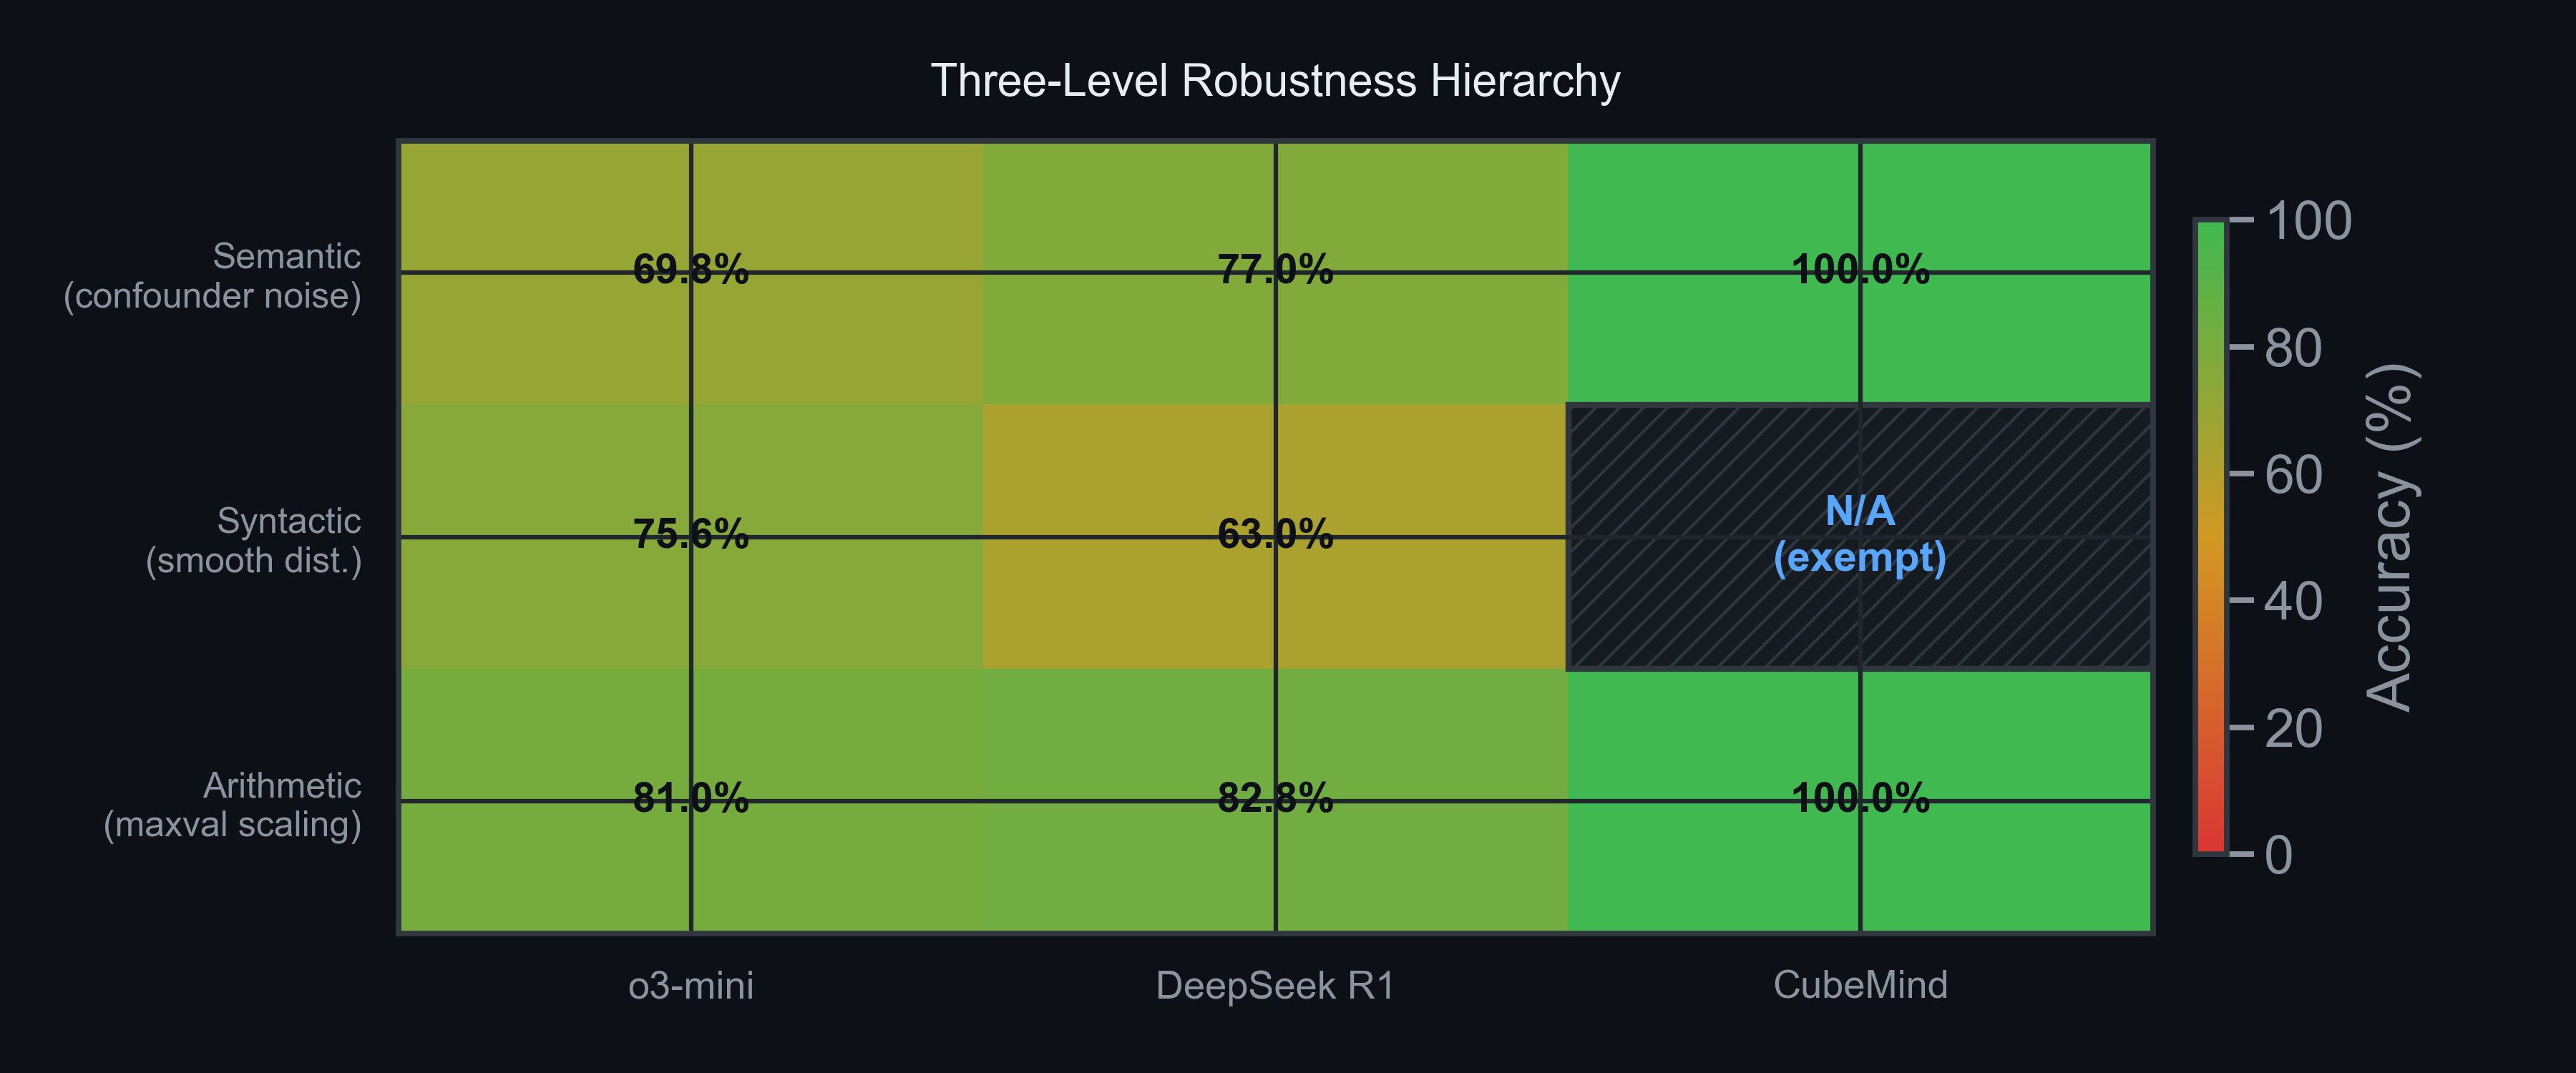
\includegraphics[width=0.75\textwidth]{paper_fig5_robustness_hierarchy.png}
    \caption{Robustness heatmap. CubeMind achieves 100\% on semantic and arithmetic axes; the syntactic axis is N/A by construction (hatched).}
    \label{fig:robustness}
\end{figure}

\subsection{Why N/A Is Stronger Than 100\%}

Smooth distributions convert discrete values into probabilistic markup (\texttt{<$p_1$::$v_1$, $p_2$::$v_2$, $p_3$::$v_3$>}) at the textual prompt level. CubeMind reads the underlying integer before any textual conversion. This is not a limitation---it is a representational level distinction: the perturbation targets the \emph{syntax} of the input, and a structured-data system is categorically exempt.

\subsection{Compounding Failure in LRMs}

Under condition~(c), both axes attack simultaneously: (1)~syntactic confusion degrades value extraction; (2)~confounder columns create an unsolvable feature selection problem for chain-of-thought; (3)~reasoning token budgets explode (18{,}482 tokens/problem). CubeMind's two immunities are independent and non-interacting.

\subsection{Implications for Benchmark Design}

I-RAVEN-X evaluates two capabilities simultaneously---rule induction and input parsing---that should be separated when comparing across system types. We propose three benchmark levels: Level~1 (clean structured data), Level~2 (noisy structured data), Level~3 (noisy textual encoding). CubeMind achieves 100\% at Level~2; LRMs face a compounding cascade at Level~3.

%----------------------------------------------------------------------
\section{Experiments}
%----------------------------------------------------------------------

\subsection{I-RAVEN-X Benchmark}

We evaluate on I-RAVEN-X with 10 confounders (200 problems per condition, seed=42, zero training).

\begin{table}[t]
\caption{I-RAVEN-X results (n=3, 10 confounders).}
\label{tab:iravenx_maxval}
\centering
\begin{tabular}{@{}lcccc@{}}
\toprule
\textbf{maxval} & \textbf{o3-mini} & \textbf{DeepSeek R1} & \textbf{CubeMind} & \textbf{Random} \\
\midrule
10   & 82.4\% & 84.0\% & \textbf{97.5\%}  & 12.5\% \\
100  & 80.6\% & 82.8\% & \textbf{99.5\%}  & 12.5\% \\
1000 & 81.0\% & 82.8\% & \textbf{100.0\%} & 12.5\% \\
\bottomrule
\end{tabular}
\end{table}

\begin{table}[t]
\caption{Condition comparison (n=3, maxval=1000). $^\dagger$Smooth distributions are prompt-level; CubeMind reads ground-truth integers (N/A by construction).}
\label{tab:iravenx_conditions}
\centering
\begin{tabular}{@{}lccc@{}}
\toprule
\textbf{Condition} & \textbf{o3-mini} & \textbf{DeepSeek R1} & \textbf{CubeMind} \\
\midrule
No confounders                       & 81.0\% & 82.8\% & \textbf{100.0\%} \\
10 confounders (SNR=$-$5.23\,dB)     & 69.8\% & 77.0\% & \textbf{100.0\%} \\
Smooth dist.\ ($p_L{=}0.51$)        & 75.6\% & 63.0\% & N/A$^\dagger$ \\
\textbf{(c) Both}                    & \textbf{17.0\%} & \textbf{23.2\%} & \textbf{100.0\%} \\
\bottomrule
\end{tabular}
\end{table}

\begin{figure}[t]
    \centering
    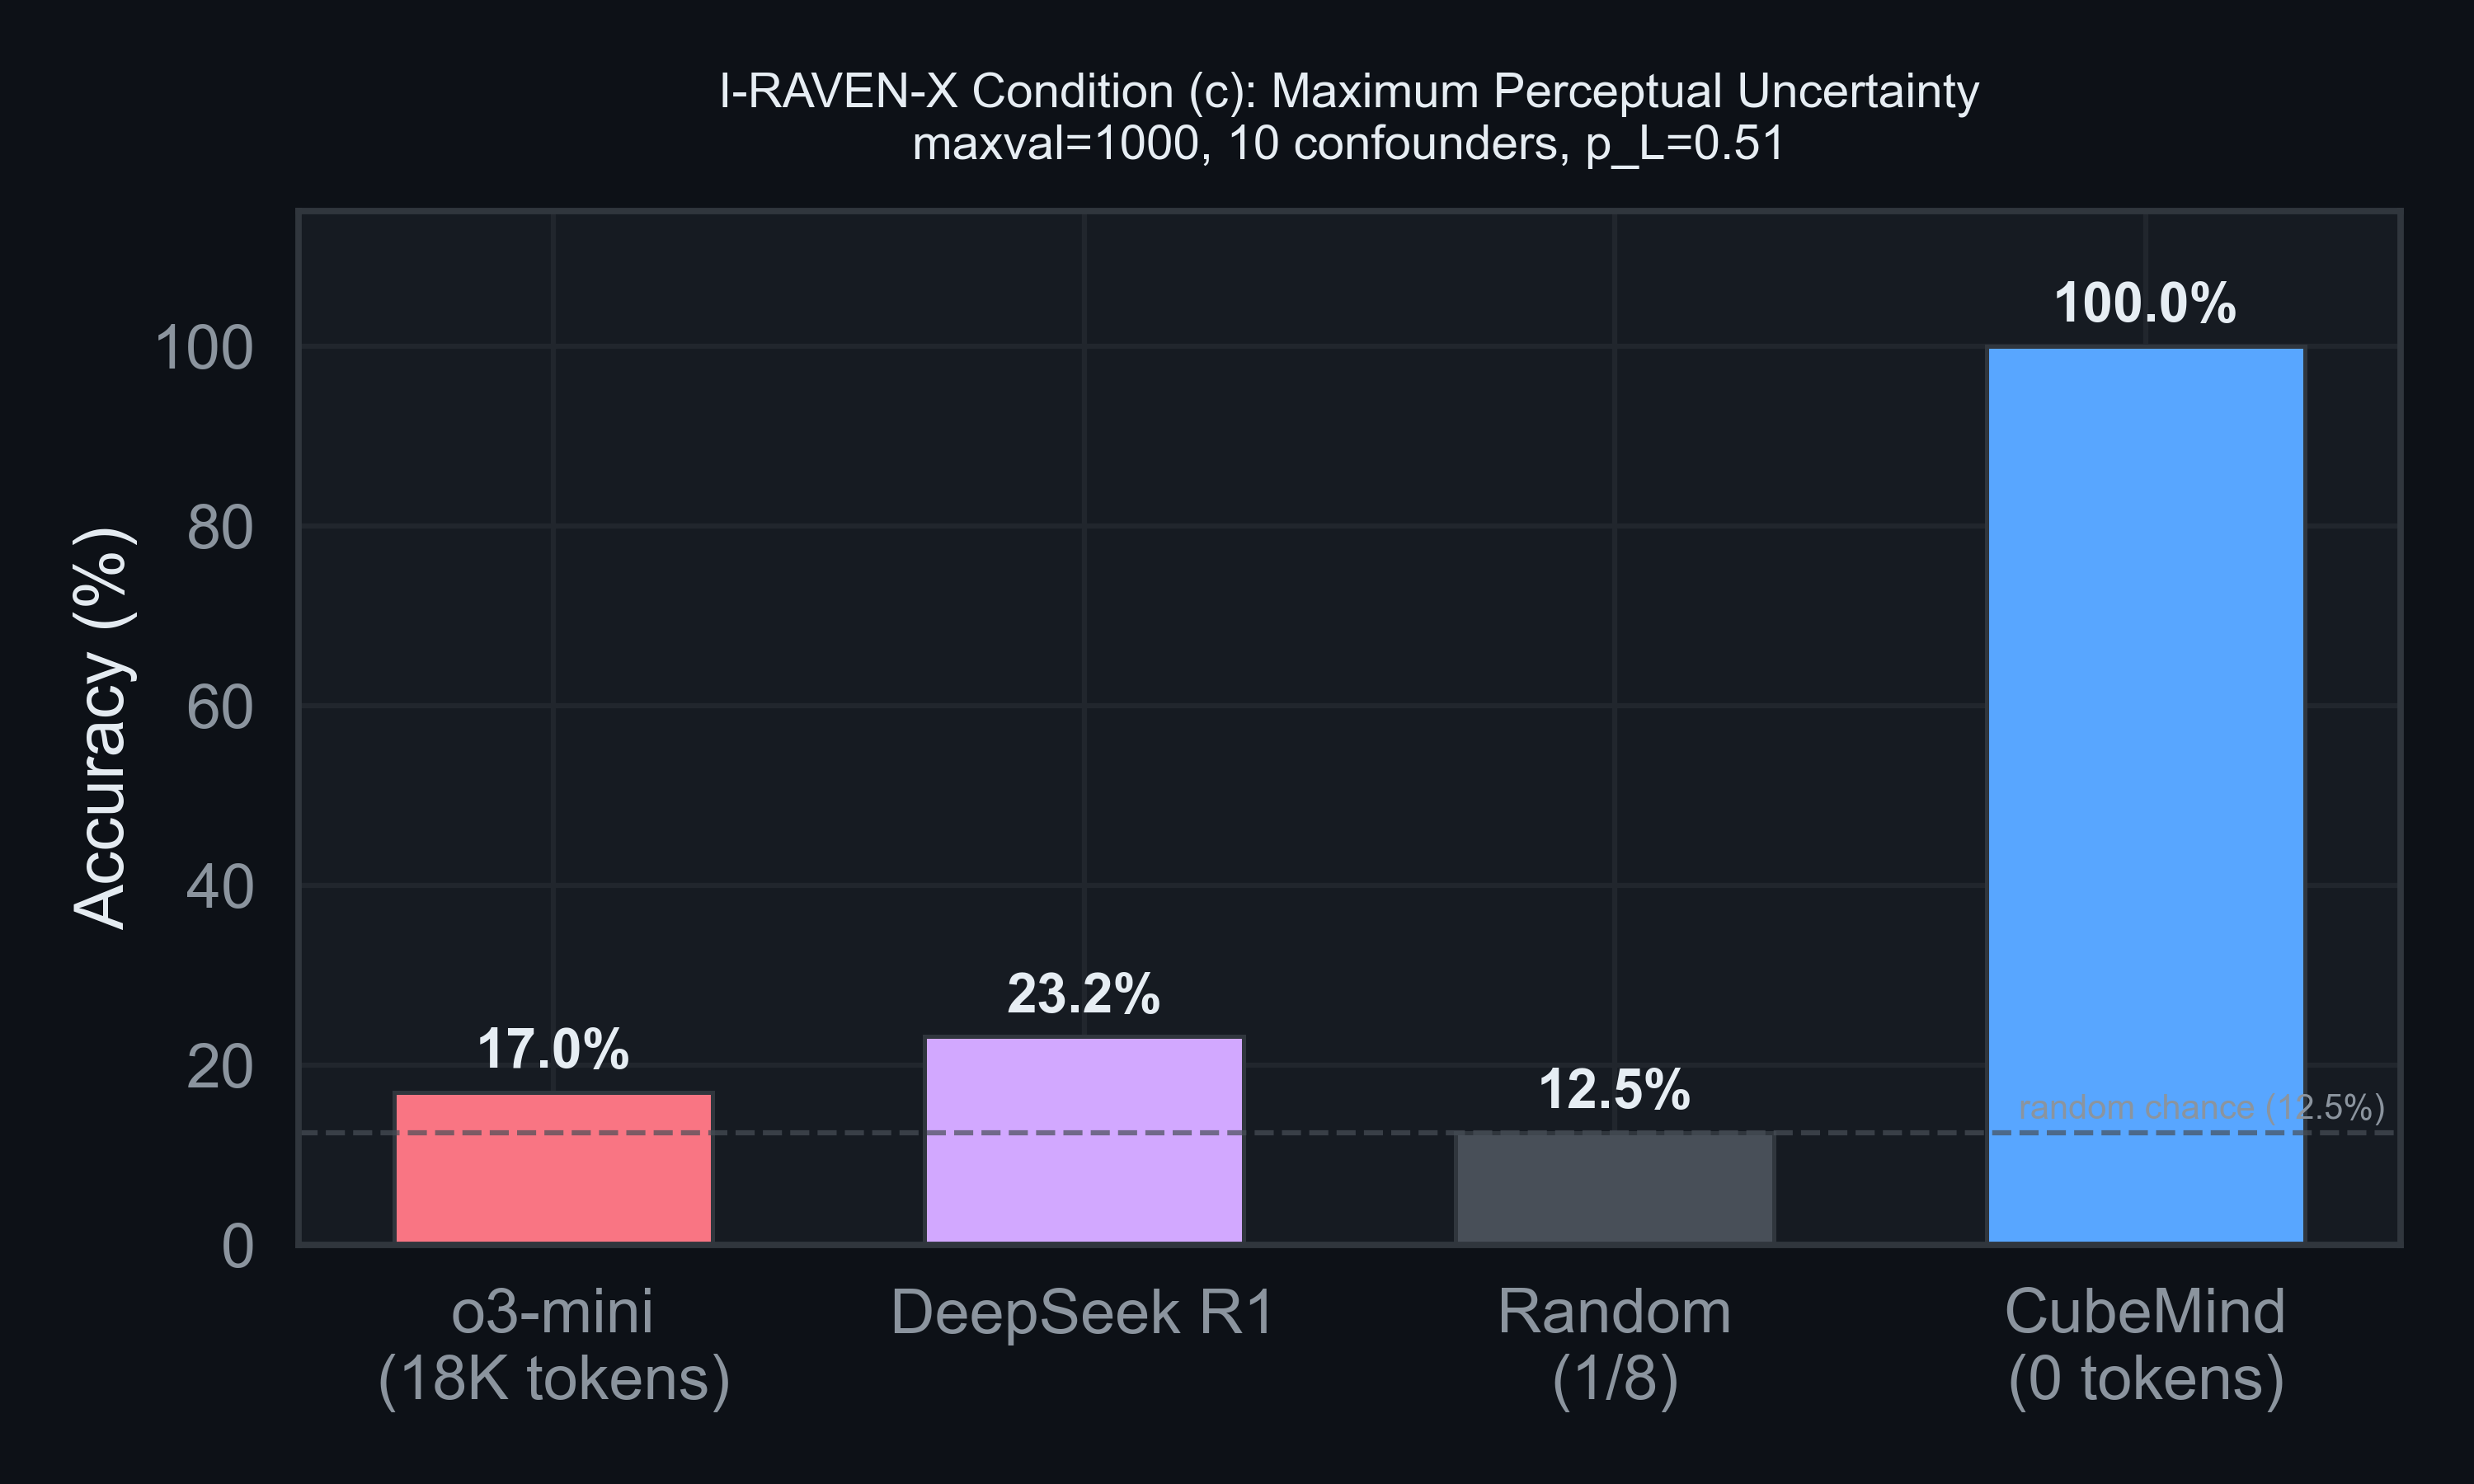
\includegraphics[width=0.48\textwidth]{paper_fig1_condition_c.png}
    \hfill
    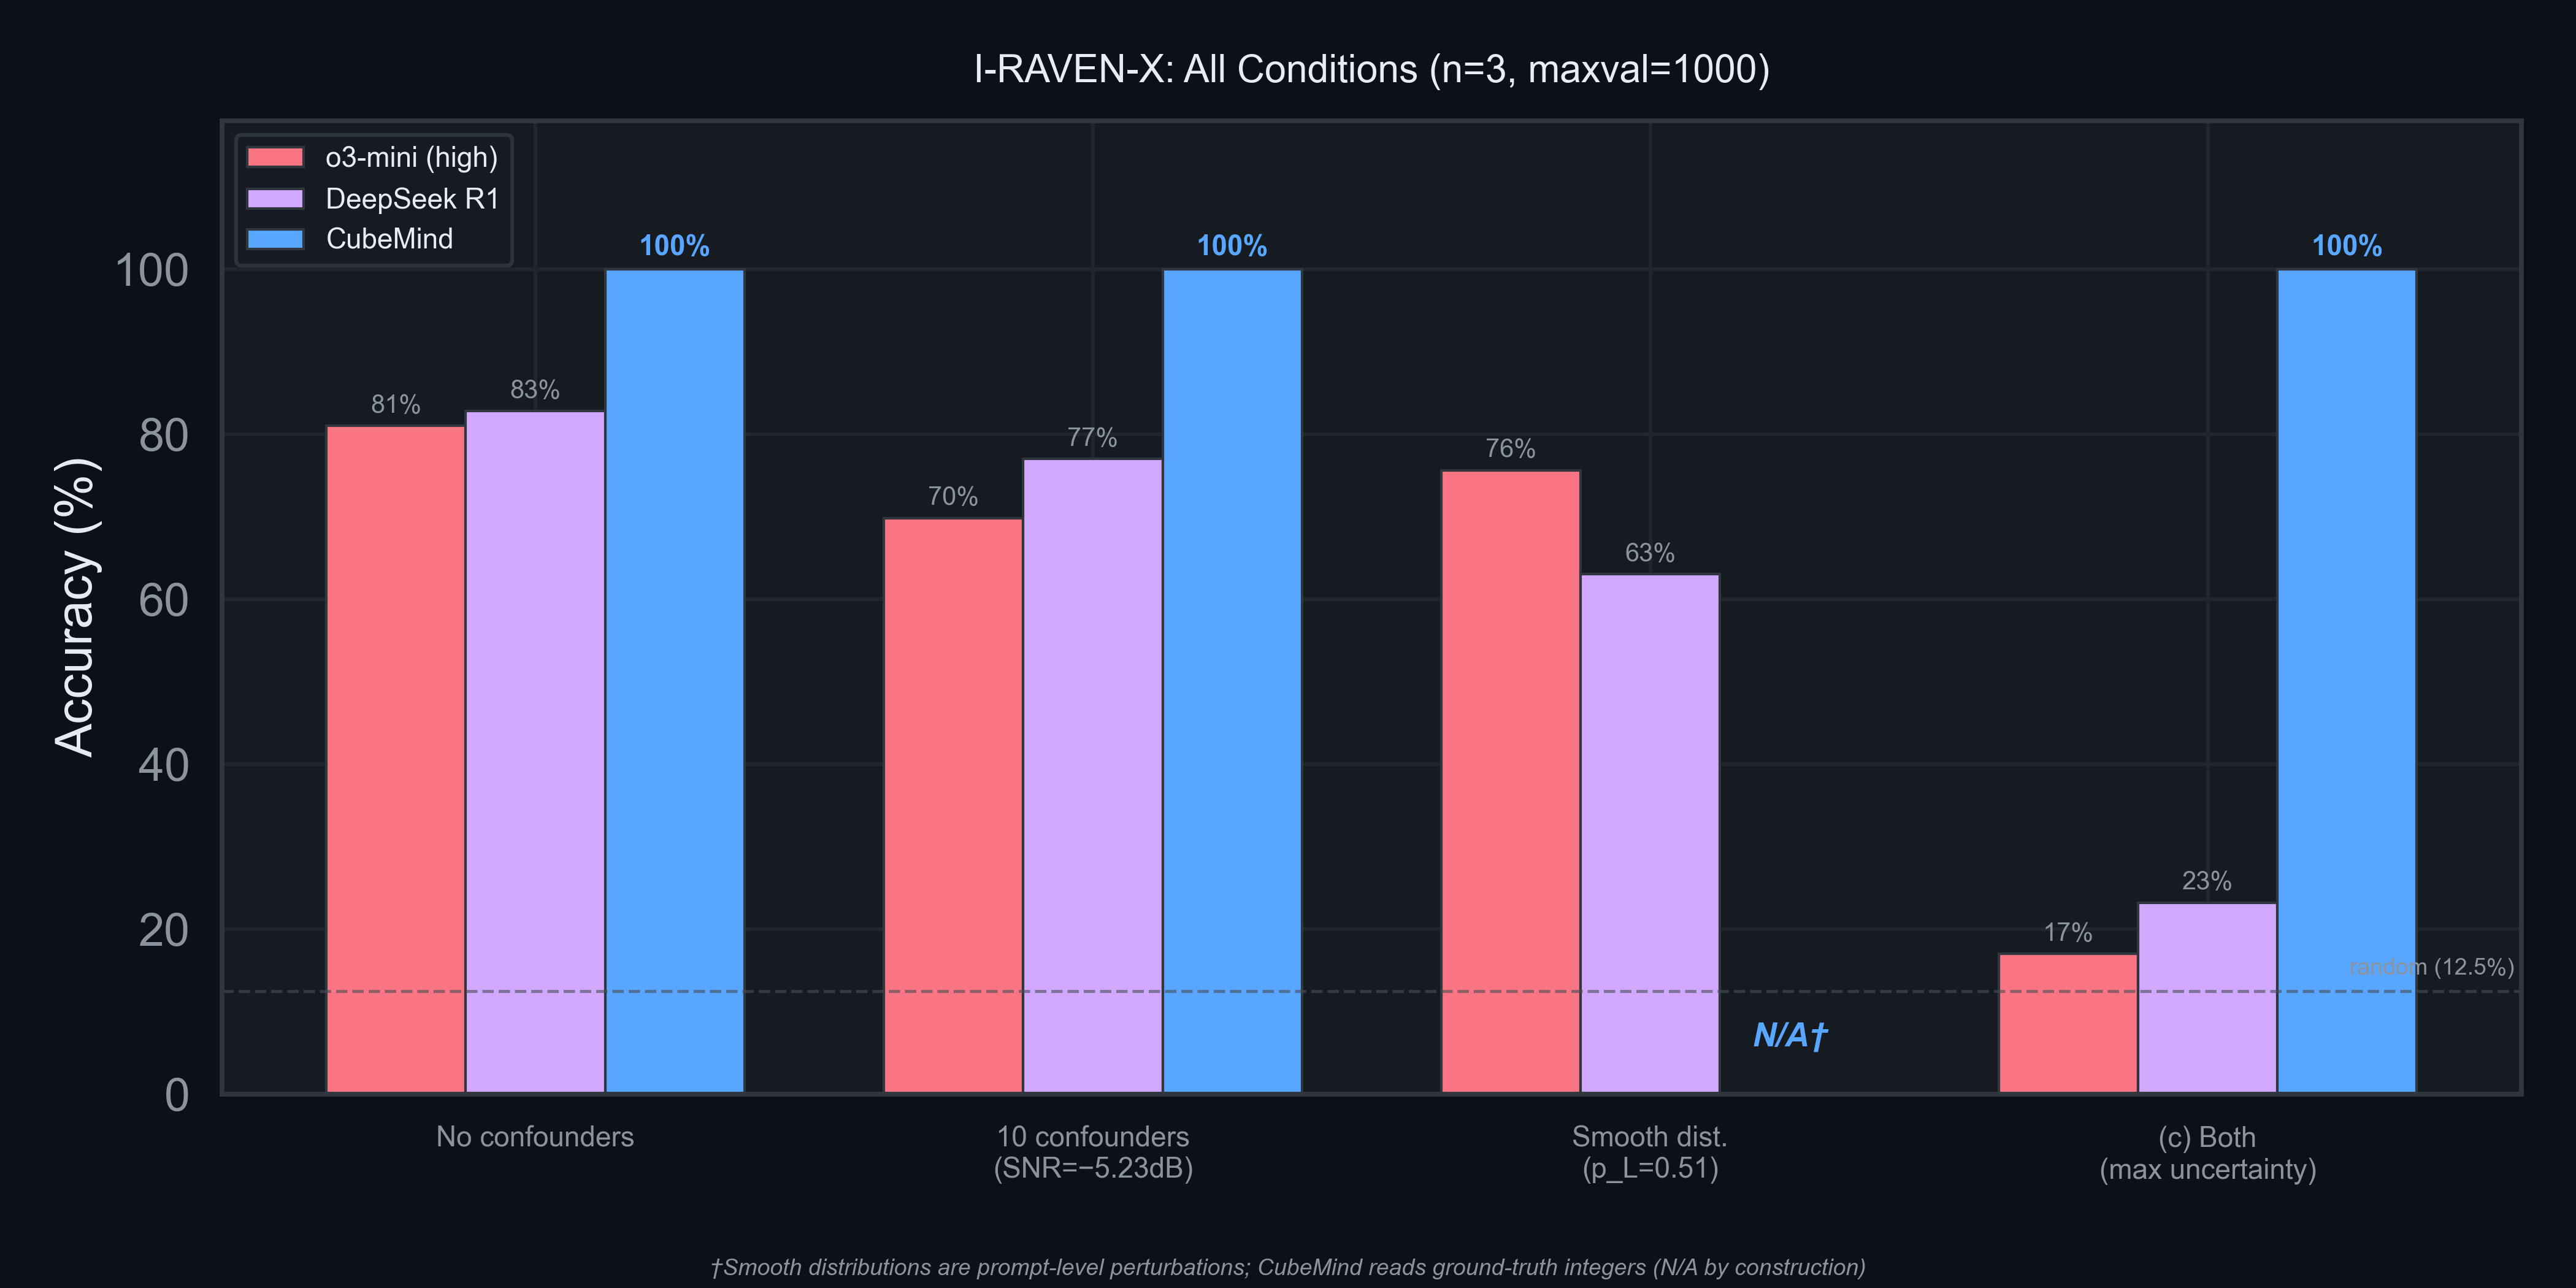
\includegraphics[width=0.48\textwidth]{paper_fig2_all_conditions.png}
    \caption{\textbf{Left:} Condition~(c) accuracy. \textbf{Right:} All conditions. The hatched N/A cell reflects categorical exemption from prompt-level perturbations.}
    \label{fig:conditions}
\end{figure}

\subsection{Standard I-RAVEN}

For completeness, Table~\ref{tab:iraven} reports results on the standard I-RAVEN benchmark (7 configurations, 200 problems each).

\begin{table}[t]
\caption{I-RAVEN results (seed=42). Mean: 90.3\% vs.\ NVSA 87.7\%~\cite{hersche2023nvsa}.}
\label{tab:iraven}
\centering
\small
\begin{tabular}{@{}lccclccc@{}}
\toprule
\textbf{Config} & \textbf{Ours} & \textbf{NVSA} & \textbf{Rand.} & \textbf{Config} & \textbf{Ours} & \textbf{NVSA} & \textbf{Rand.} \\
\midrule
Center  & 97.5 & $\sim$98 & 12.5 & L--R   & 98.0 & $\sim$96 & 12.5 \\
$2{\times}2$ & 82.0 & $\sim$84 & 12.5 & U--D   & 96.0 & $\sim$95 & 12.5 \\
$3{\times}3$ & 81.5 & $\sim$83 & 12.5 & O-I-C  & \textbf{100.0} & $\sim$99 & 12.5 \\
       &      &          &      & O-I-G  & 77.0 & $\sim$71 & 12.5 \\
\midrule
\multicolumn{4}{@{}l}{\textbf{Mean: 90.3\%}} & \multicolumn{4}{l@{}}{\textbf{NVSA: 87.7\%}} \\
\bottomrule
\end{tabular}
\end{table}

\subsection{Efficiency}

\begin{table}[t]
\caption{Efficiency under condition~(c). The gap is qualitative, not quantitative.}
\label{tab:efficiency}
\centering
\begin{tabular}{@{}lcc@{}}
\toprule
\textbf{Metric} & \textbf{o3-mini} & \textbf{CubeMind} \\
\midrule
Tokens/problem & 18{,}482 & 0 \\
Wall-clock (200) & $\sim$hours & \textbf{1.86\,s} \\
Training & Massive pretraining & None \\
Accuracy & 17.0\% & \textbf{100.0\%} \\
\bottomrule
\end{tabular}
\end{table}

\subsection{Value Range Invariance}

CubeMind's accuracy \emph{increases} with maxval (97.5\% $\rightarrow$ 99.5\% $\rightarrow$ 100.0\% for 10/100/1000)---the opposite of LRM degradation. Larger ranges reduce coincidental matches, confirming genuine rule induction over memorization (Figure~\ref{fig:maxval}).

\begin{figure}[t]
    \centering
    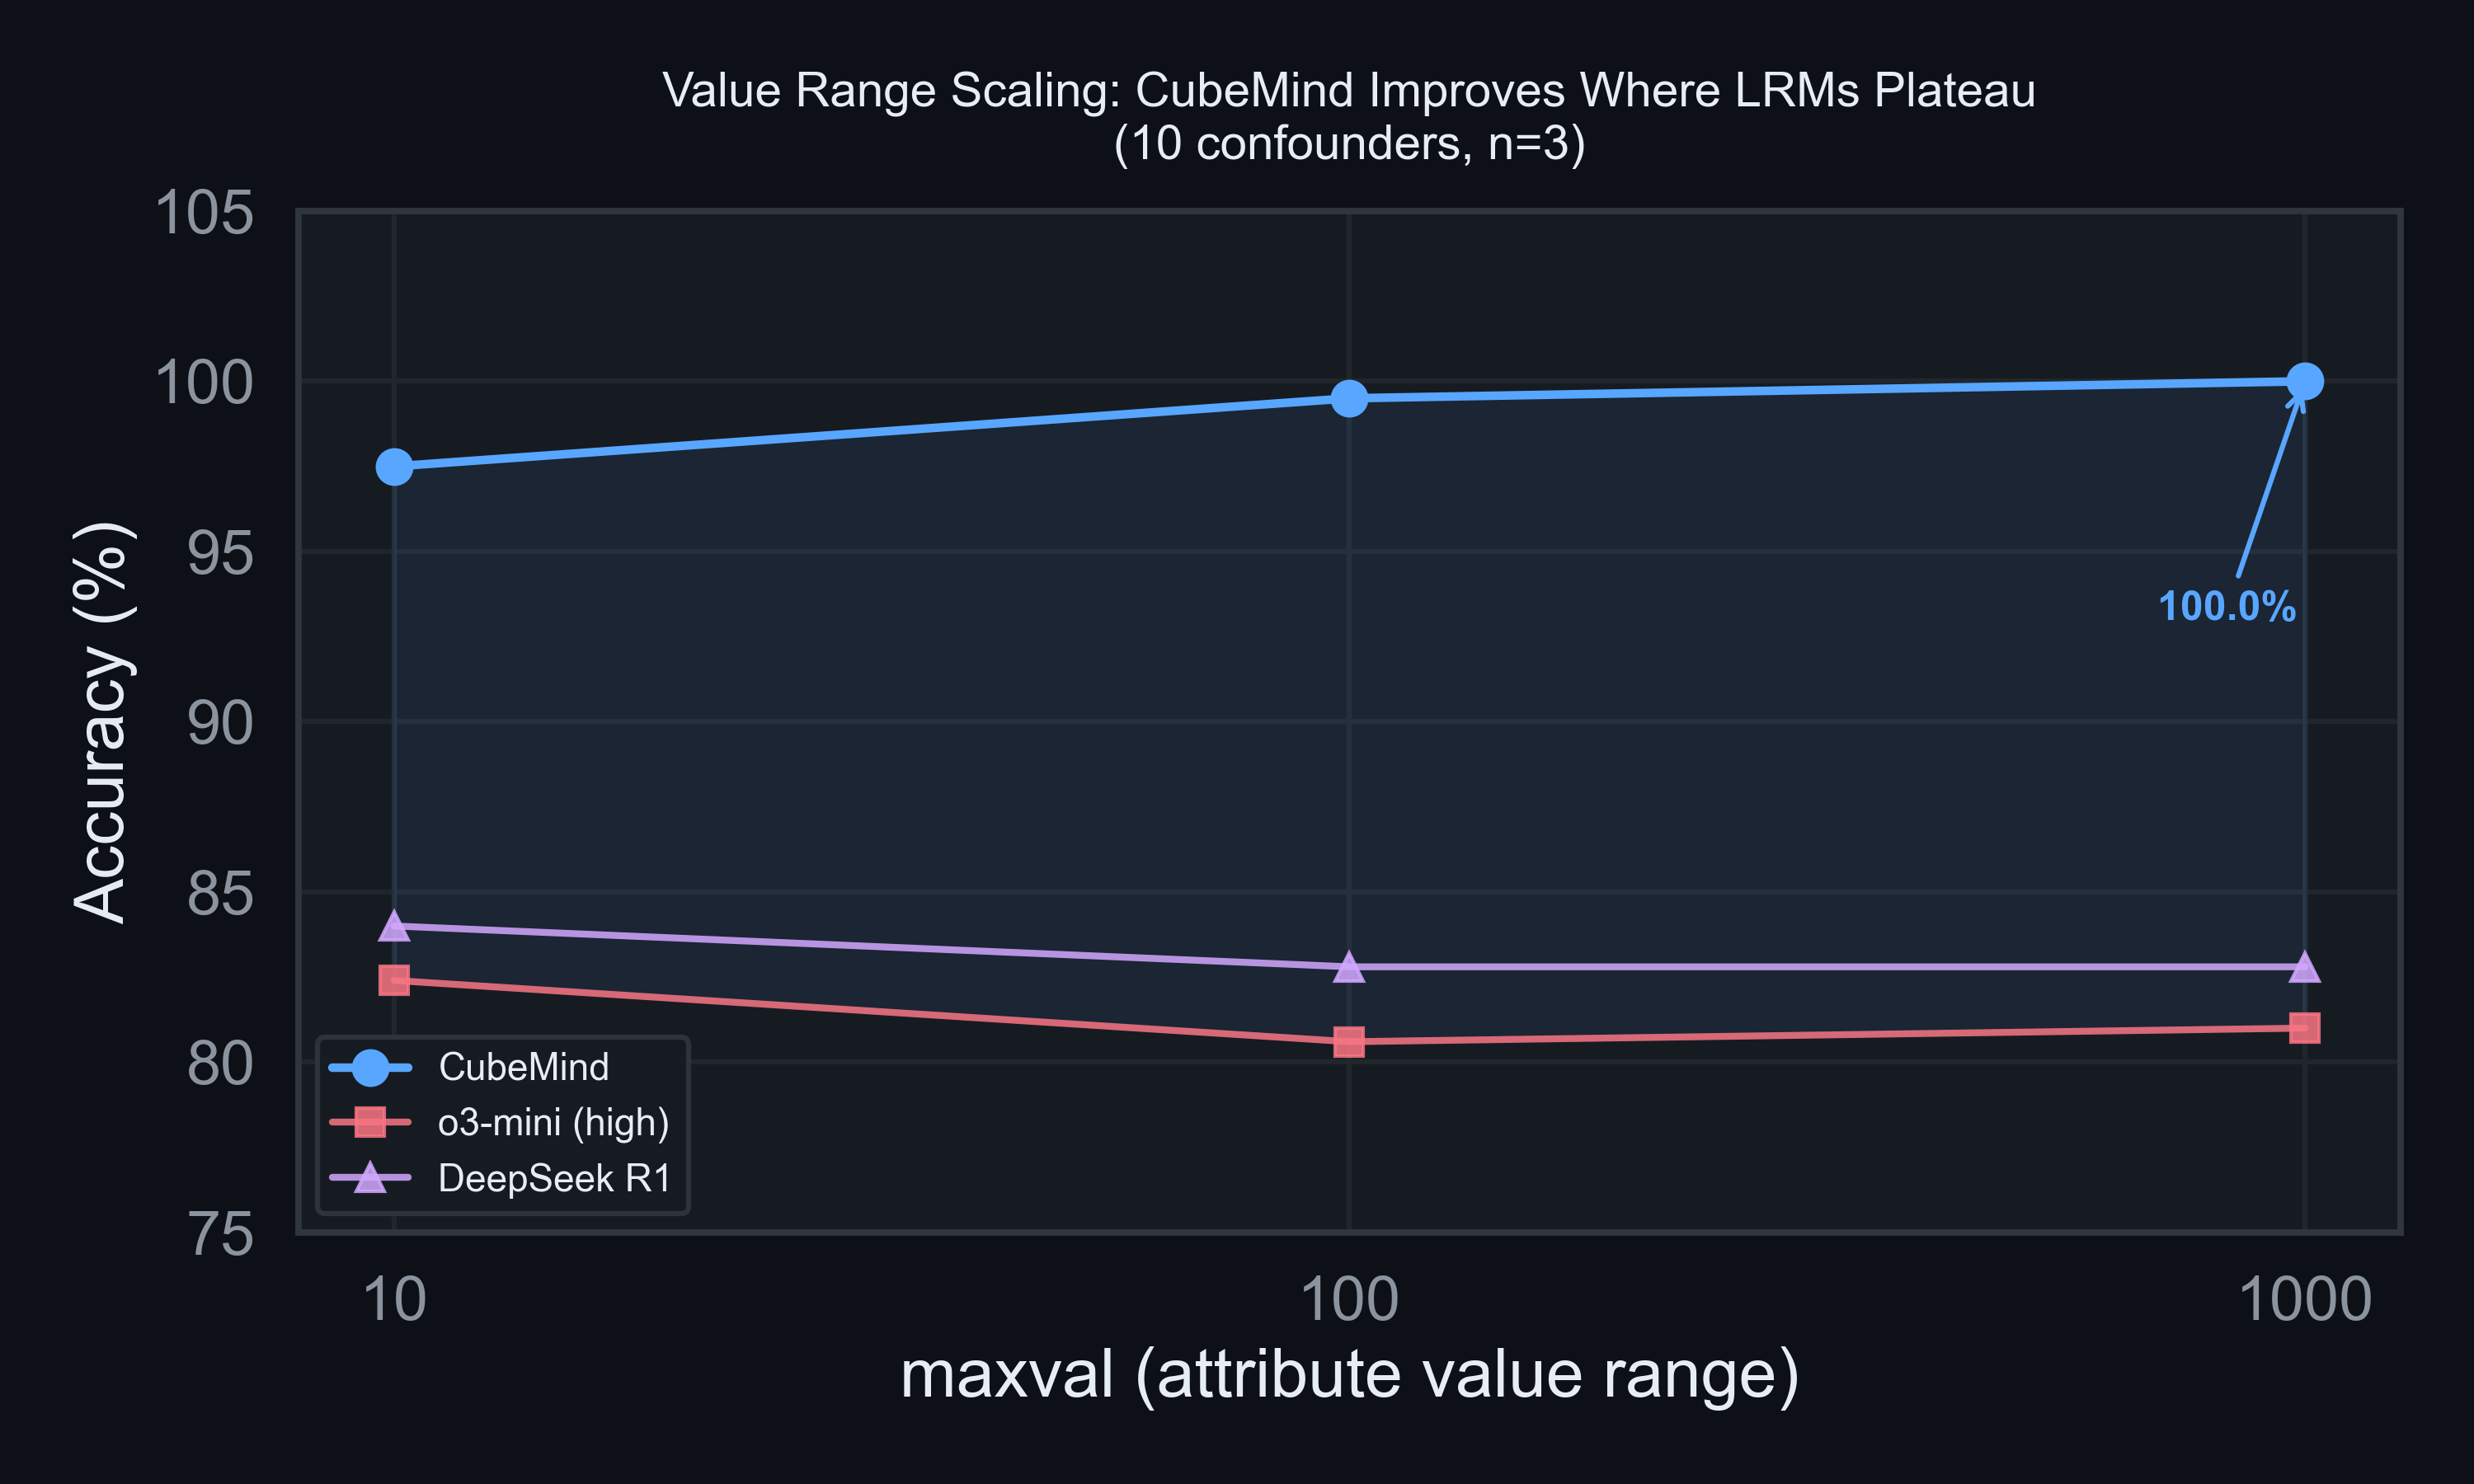
\includegraphics[width=0.6\textwidth]{paper_fig3_maxval_scaling.png}
    \caption{CubeMind accuracy increases with maxval while LRMs plateau.}
    \label{fig:maxval}
\end{figure}

\subsection{Limitation: Large Grids}

On $10{\times}10$ grids (99 context panels), accuracy drops to 41.0\%. Distribute-Three detection fails (0\%) because the current detector assumes 3-row structure. Extending to variable-length rows is future work.

%----------------------------------------------------------------------
\section{Related Work}
%----------------------------------------------------------------------

\paragraph{Neuro-Vector-Symbolic Architectures.}
NVSA~\cite{hersche2023nvsa} pioneered VSA-based abstract reasoning (87.7\% on I-RAVEN). CubeMind extends this with deterministic integer-domain detectors and HMM ensemble tiebreaking (90.3\%). RESOLVE~\cite{resolve2026} performs relational reasoning in hyperdimensional spaces but does not address perceptual uncertainty.

\paragraph{Large Reasoning Models.}
o3-mini~\cite{openai2025o3mini} and DeepSeek~R1~\cite{deepseek2025r1} achieve $\sim$82\% on clean I-RAVEN-X but collapse under perturbation because the reasoning budget is consumed by input parsing.

\paragraph{Active Inference.}
Applied to robotics~\cite{world_models_robotics2023} and RL~\cite{deep_active_inference2026}, but not to abstract visual reasoning. Our HMM ensemble divergence as an EFE proxy is, to our knowledge, the first application to RPM-style benchmarks.

\paragraph{Robustness.}
Neural Prediction Errors~\cite{neural_prediction2026} use surprise signals; the Reasoning Topology framework~\cite{huang2026reasoning} proves graph topology determines reasoning quality. We show representational level is the primary determinant under perceptual uncertainty.

%----------------------------------------------------------------------
\section{Discussion}
%----------------------------------------------------------------------

\paragraph{Is CubeMind ``cheating''?}
Reading structured JSON is not bypassing the problem---Raven's Matrices are fundamentally about rule induction from structured attributes. The textual encoding is an artifact of how LRMs consume input, not an inherent property of the task.

\paragraph{Generalization.}
The scored-attribute-set principle is not RPM-specific. The same VSA binding machinery extends to neural vision (binding frame attributes into episode hypervectors), temporal memory (permuted bundles over timesteps), and cross-modal zero-shot transfer (shared binding keys across modalities). See Appendix~\ref{app:generalization} for details.

\paragraph{Many-worlds decision making.}
The broader architecture includes a DecisionOracle (Appendix~\ref{app:decision_oracle}) whose $N$-world personality ensemble implements the ``probabilistic superposition over competing world models'' that Sicking et al.~\cite{sicking2026iravenx} identify as absent in LRMs. Evaluating this component on reasoning benchmarks is future work.

%----------------------------------------------------------------------
\section{Conclusion}
%----------------------------------------------------------------------

CubeMind achieves 100.0\% on I-RAVEN-X under maximum perceptual uncertainty---the condition where LRMs score near random chance. This is not due to superior learning but to operating at the correct representational level: ground-truth integers rather than tokenized text, scored attribute sets rather than learned attention, and exact arithmetic rather than stochastic token generation. The three-level robustness hierarchy (semantic immunity, syntactic exemption, arithmetic invariance) explains why scaling tokens cannot solve abstract reasoning robustness: the failure is representational, not computational.

%----------------------------------------------------------------------
\newpage
\appendix

\section{Generalization of the VSA Binding Principle}
\label{app:generalization}

The I-RAVEN-X result is a special case of a general principle: \textbf{ground representations before reasoning}. The same VSA bind/bundle/permute operations apply across domains:

\paragraph{Neural vision.} Per-frame color warmth, hue, and brightness are structured attributes bound into episode hypervectors:
\[\texttt{episode} = \text{bind}(\text{object}, \text{bind}(\text{position}, \text{bind}(\text{color}, \text{frame})))\]
Confounder robustness transfers: the scored attribute set is whatever the encoder abstracts; irrelevant pixels are ignored.

\paragraph{Timelines.} A timeline is a permuted bundle $\text{Memory} = \sum_t \rho^t(\text{episode}(t))$. Similarity queries, novelty detection (cosine distance from the bundle), and restructuration (re-binding with updated time vectors) all operate in the same algebra.

\paragraph{Zero-shot cross-modal transfer.} Because VSA binding is compositional, a concept learned in one modality transfers via shared binding keys. A visual ``explosion'' vector can be queried from text features without fine-tuning---structural alignment at the hyperdimensional level.

\paragraph{Multi-attribute reasoning.} The pattern generalizes: (1)~assign type-specific encoders, (2)~bind into episode vectors, (3)~reason over bindings. The system never translates across modalities via text.

\paragraph{DecisionOracle hierarchy.}
\begin{itemize}
    \item \textbf{I-RAVEN-X}: integer attributes + deterministic detectors = crisp world model
    \item \textbf{Video}: frame attributes + neurochemical state = episodic VSA world model
    \item \textbf{Causal graphs}: events + entity/time = symbolic world model
    \item \textbf{DecisionOracle}: all above + $N$ personality-modulated world dynamics via shared hypernetwork
\end{itemize}

\begin{figure}[h]
    \centering
    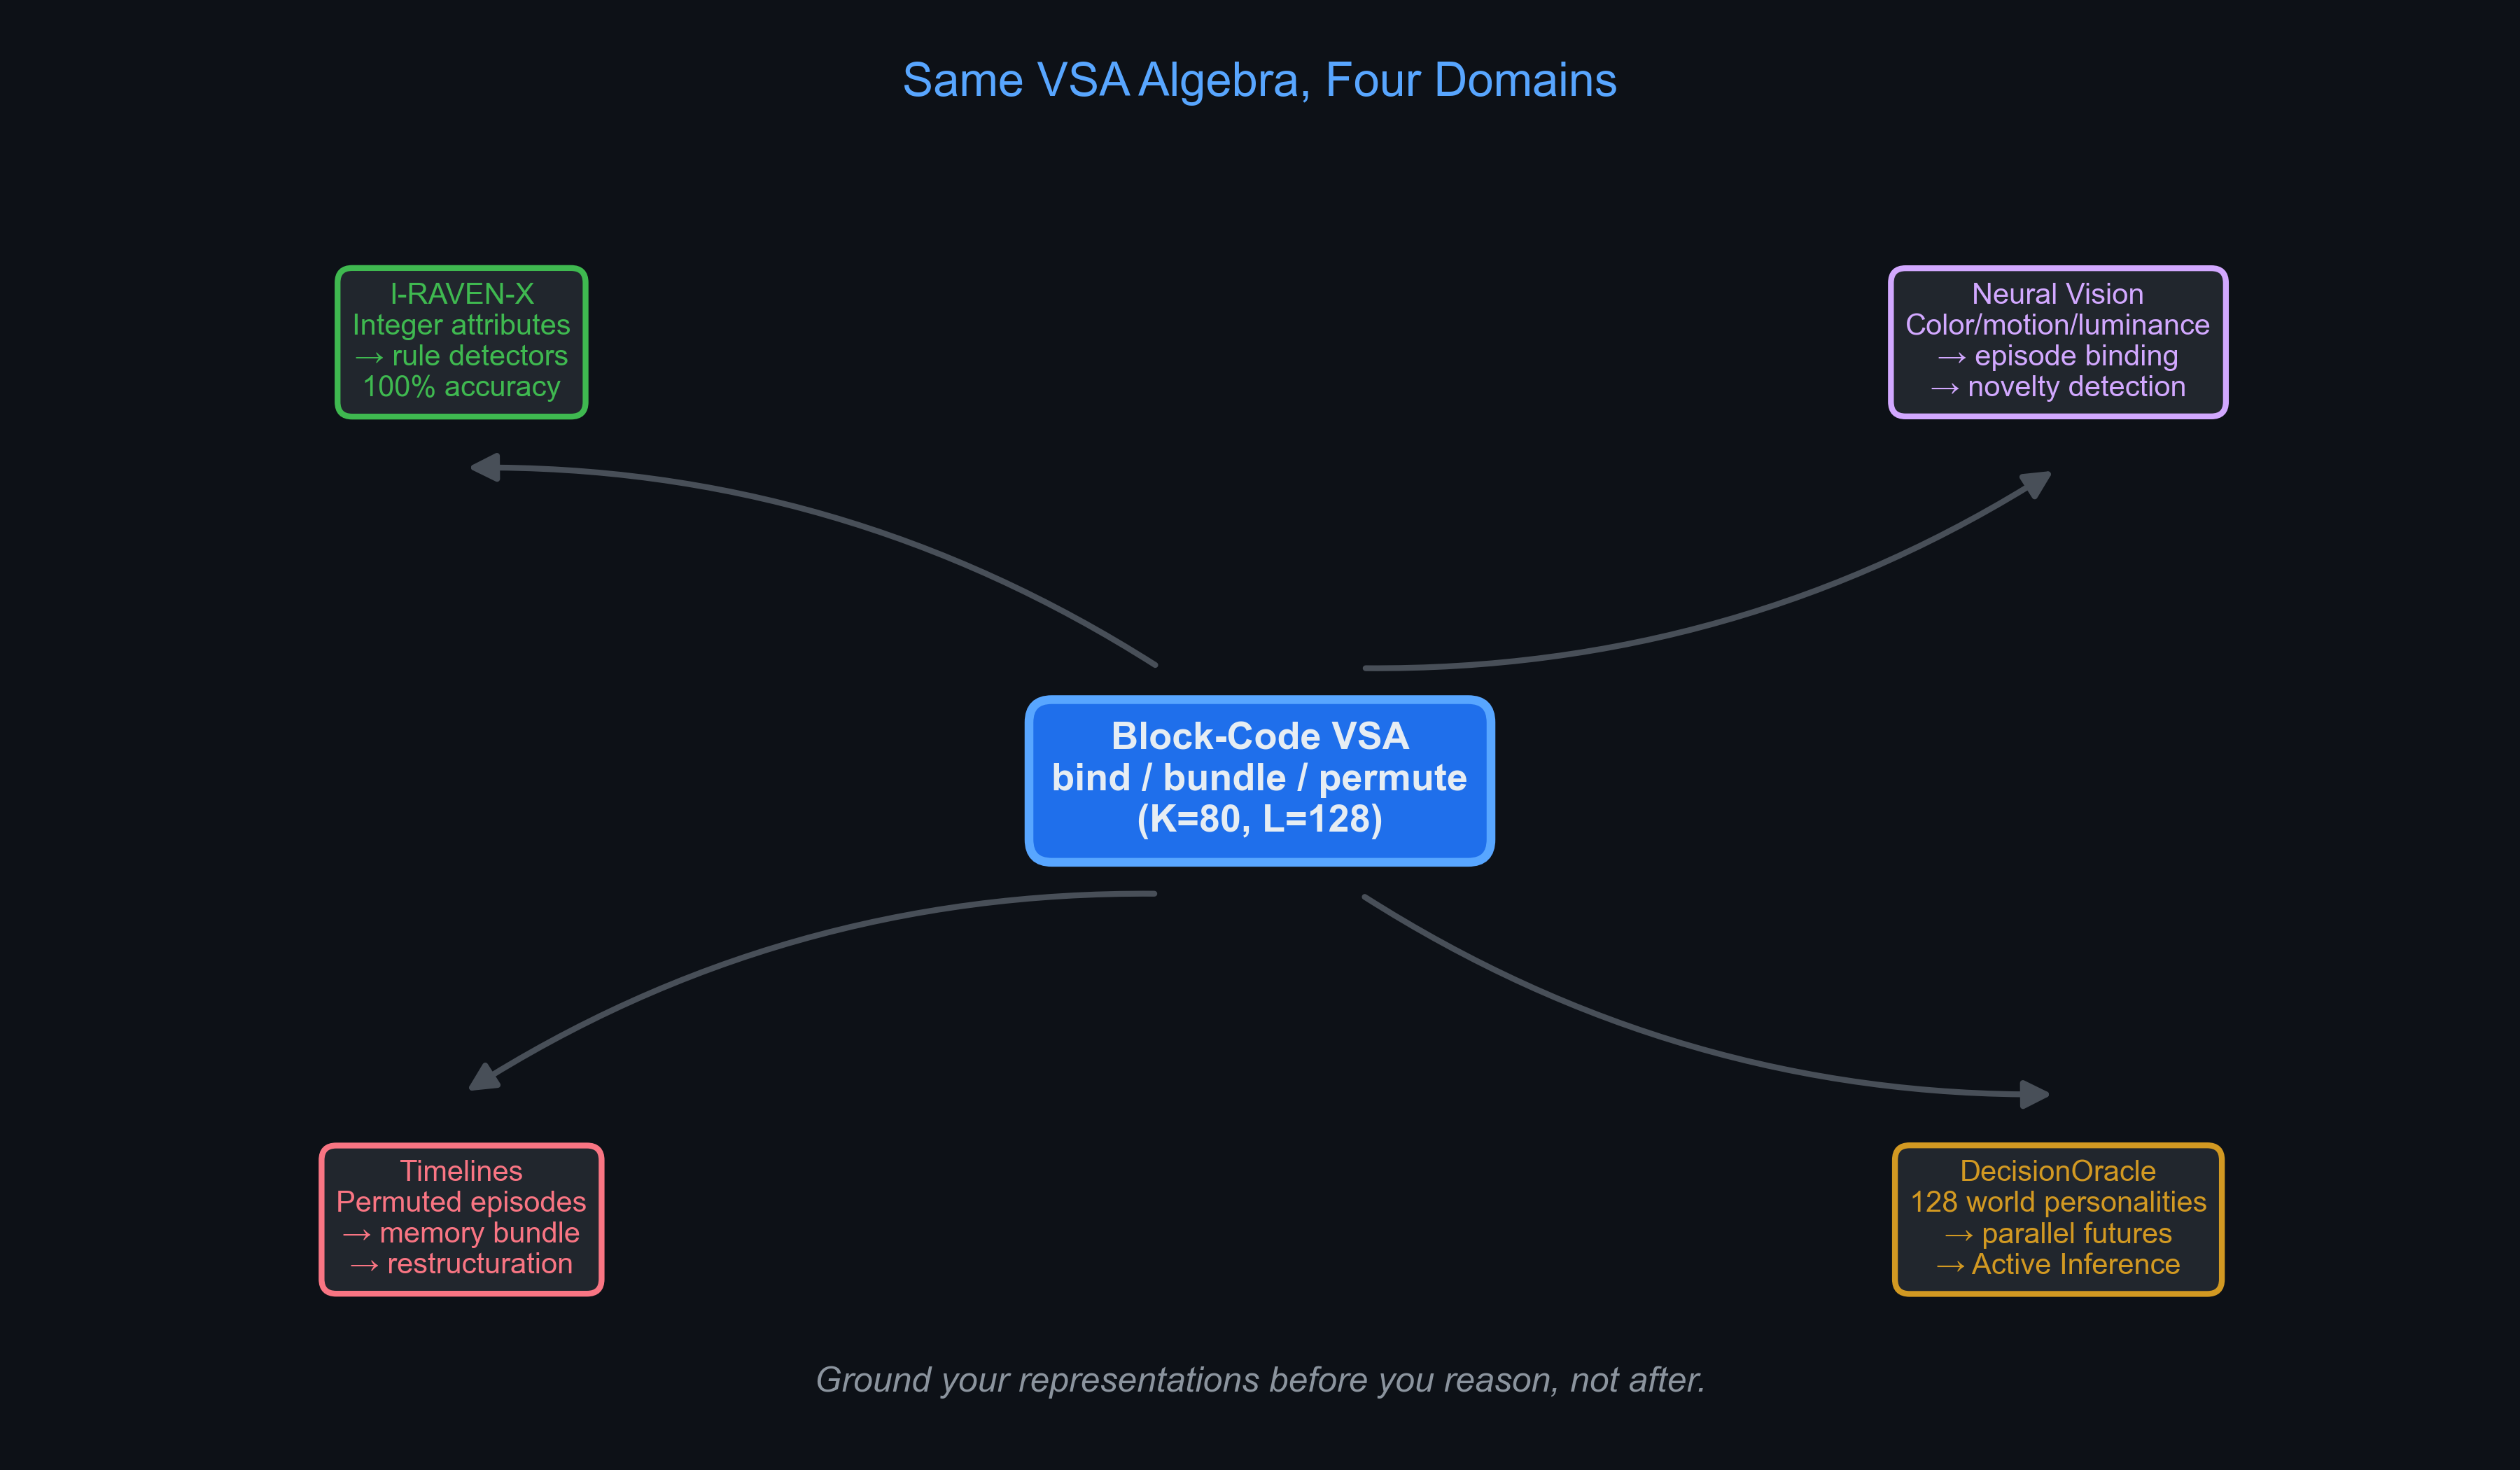
\includegraphics[width=0.75\textwidth]{paper_fig7_vsa_hierarchy.png}
    \caption{Same block-code VSA operations underlie all four domains.}
    \label{fig:vsa_hierarchy}
\end{figure}

\section{DecisionOracle: Many-Worlds Active Inference}
\label{app:decision_oracle}

The DecisionOracle module extends the Active Inference interpretation to general-purpose decision making. A single hypernetwork (HYLA) combined with $N$ ``world personality'' vectors defines an ensemble of generative models $p_\omega(s_{t+1} \mid s_t, a_t)$, one per world~$\omega$. For a given state--action pair, DecisionOracle produces $N$ candidate futures with plausibility $P_\omega \geq 0$ (epistemic) and Q-values $Q_\omega \in \mathbb{R}$ (pragmatic). The \texttt{top\_k} operator combines these into a composite score, implementing soft EFE minimization: actions are preferred when they lead to futures that are both likely and high-value. This is memory-efficient (${\sim}2$\,MB for 128 worlds) because diversity comes from personality-binding through a shared hypernetwork.

\begin{figure}[h]
    \centering
    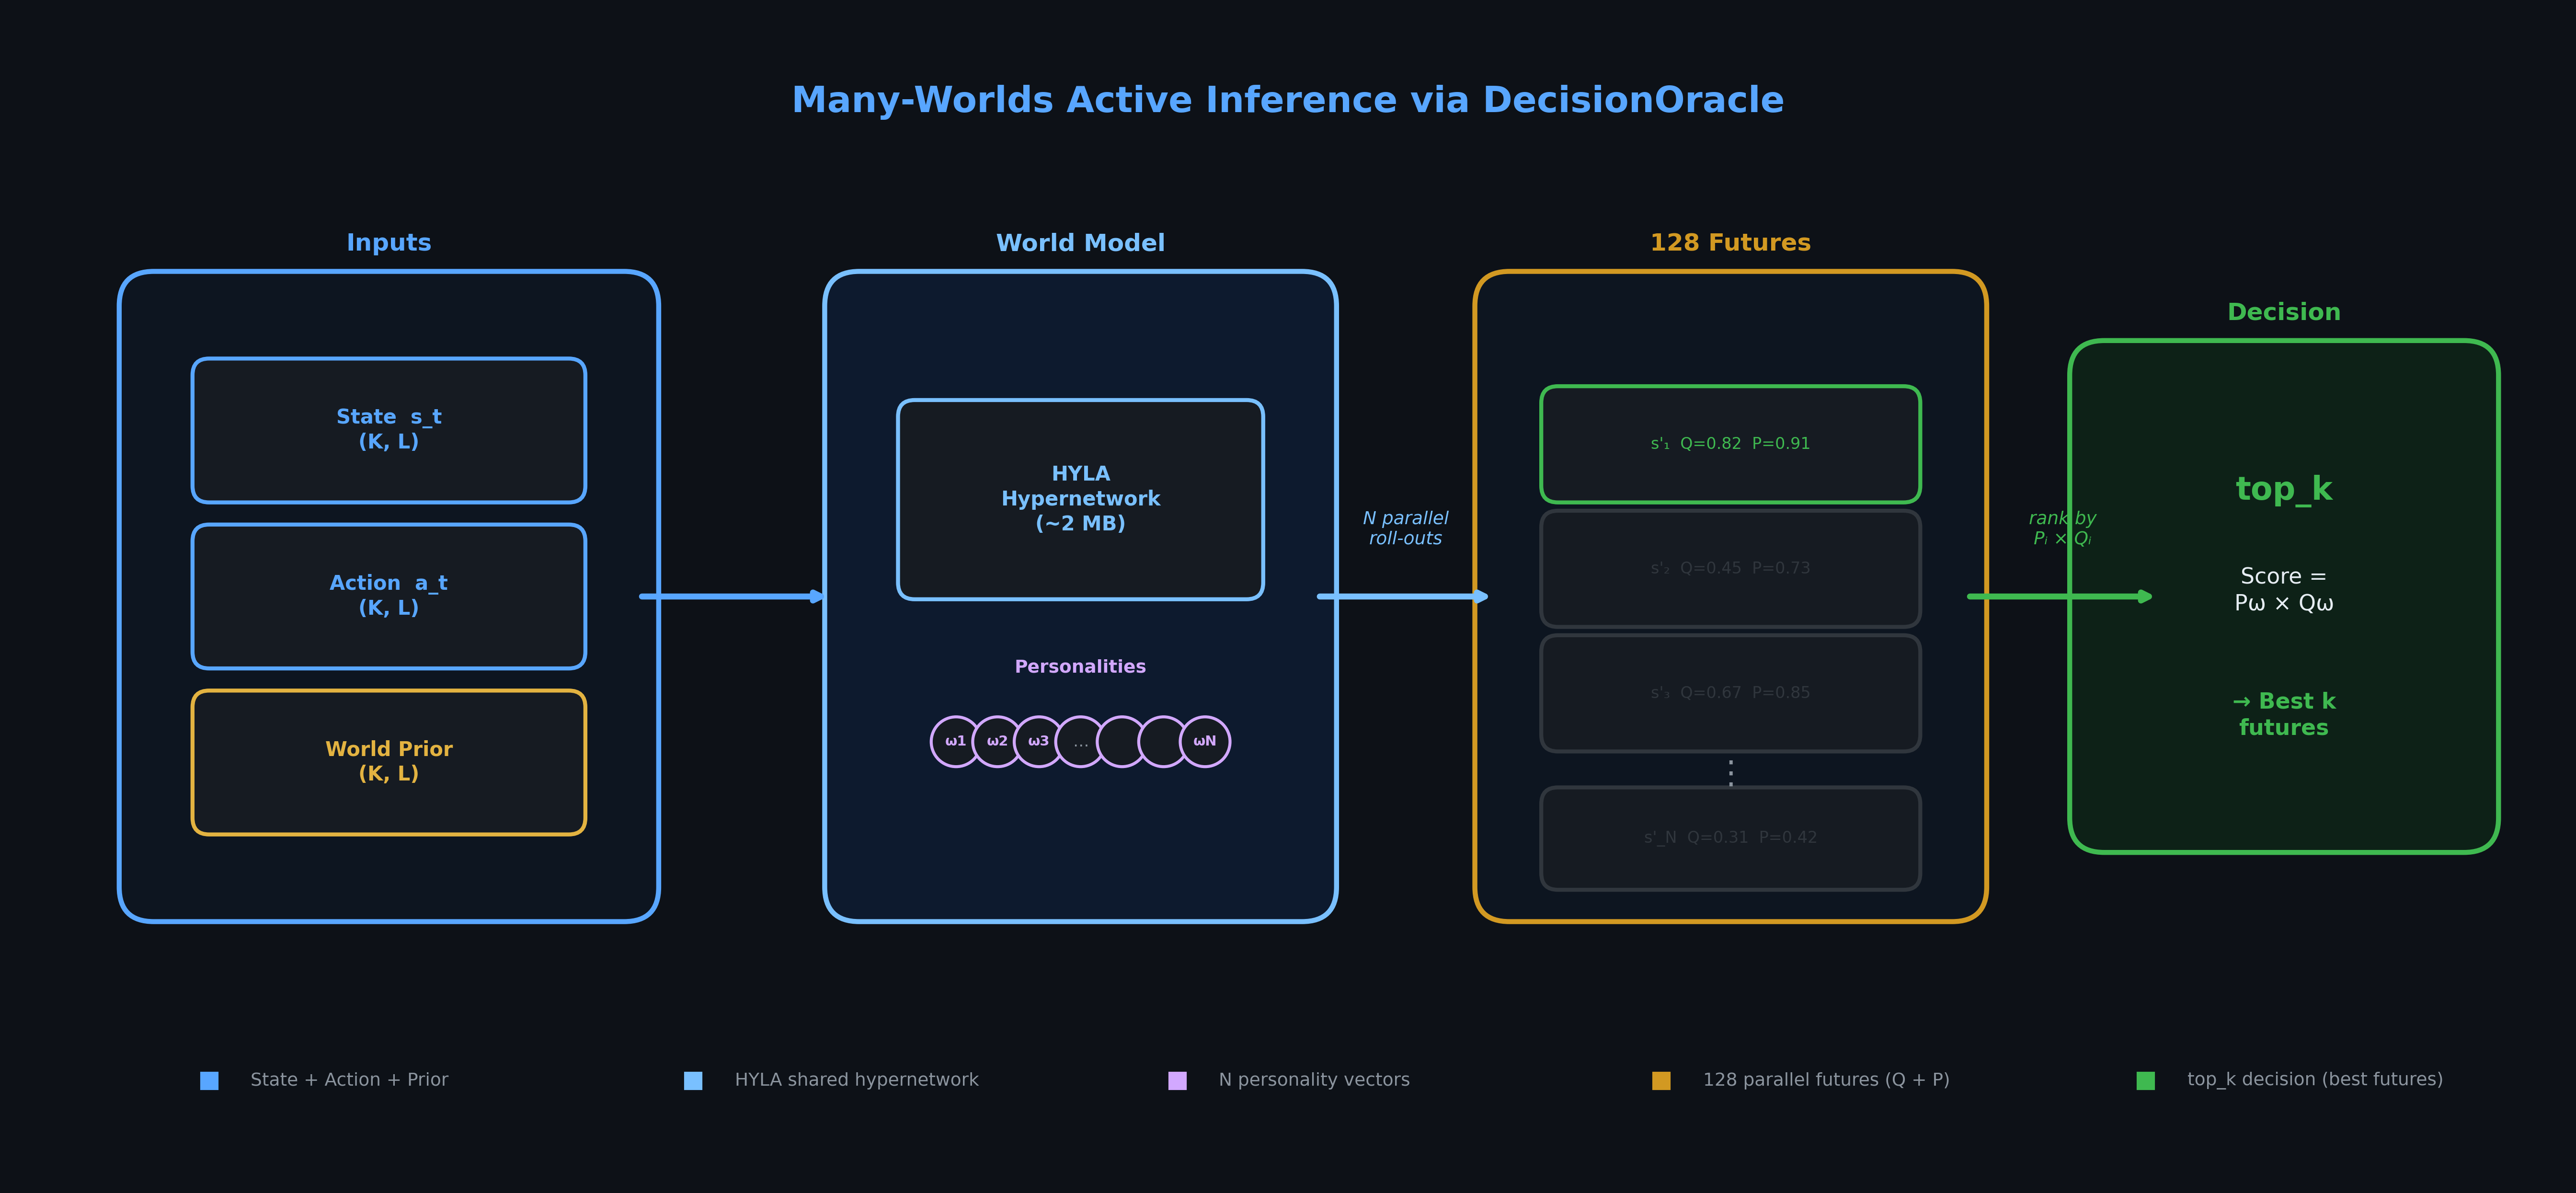
\includegraphics[width=\textwidth]{paper_fig8_many_worlds.png}
    \caption{DecisionOracle pipeline. A single HYLA hypernetwork modulated by $N$ personality vectors produces $N$ parallel futures with Q-values (pragmatic) and plausibility scores (epistemic). The \texttt{top\_k} operator implements soft EFE minimization.}
    \label{fig:many_worlds}
\end{figure}

This component is not used in the I-RAVEN-X evaluation reported in this paper. It is included to illustrate how the same VSA algebra (bind, bundle, permute) extends from deterministic rule detection to probabilistic many-worlds decision making without changing the underlying representational machinery.

\section{Implementation Details}
\label{app:implementation}

All experiments run on a single NVIDIA L4 GPU (24\,GB) in Google Colab. The codebase is Python~3.12 with critical paths in C++/Vulkan compute shaders via a 3-level GPU fallback. No API calls, no training data. Development uses an AMD RX~6750~XT (12\,GB)---all results reproduce on both backends.

All benchmarks use fixed seeds (42). The I-RAVEN-X generation code is from the public repository with our \texttt{n\_confounders} extension. Source will be released upon acceptance.

\section{Double Binding Diagram}
\label{app:double_binding}

\begin{figure}[h]
    \centering
    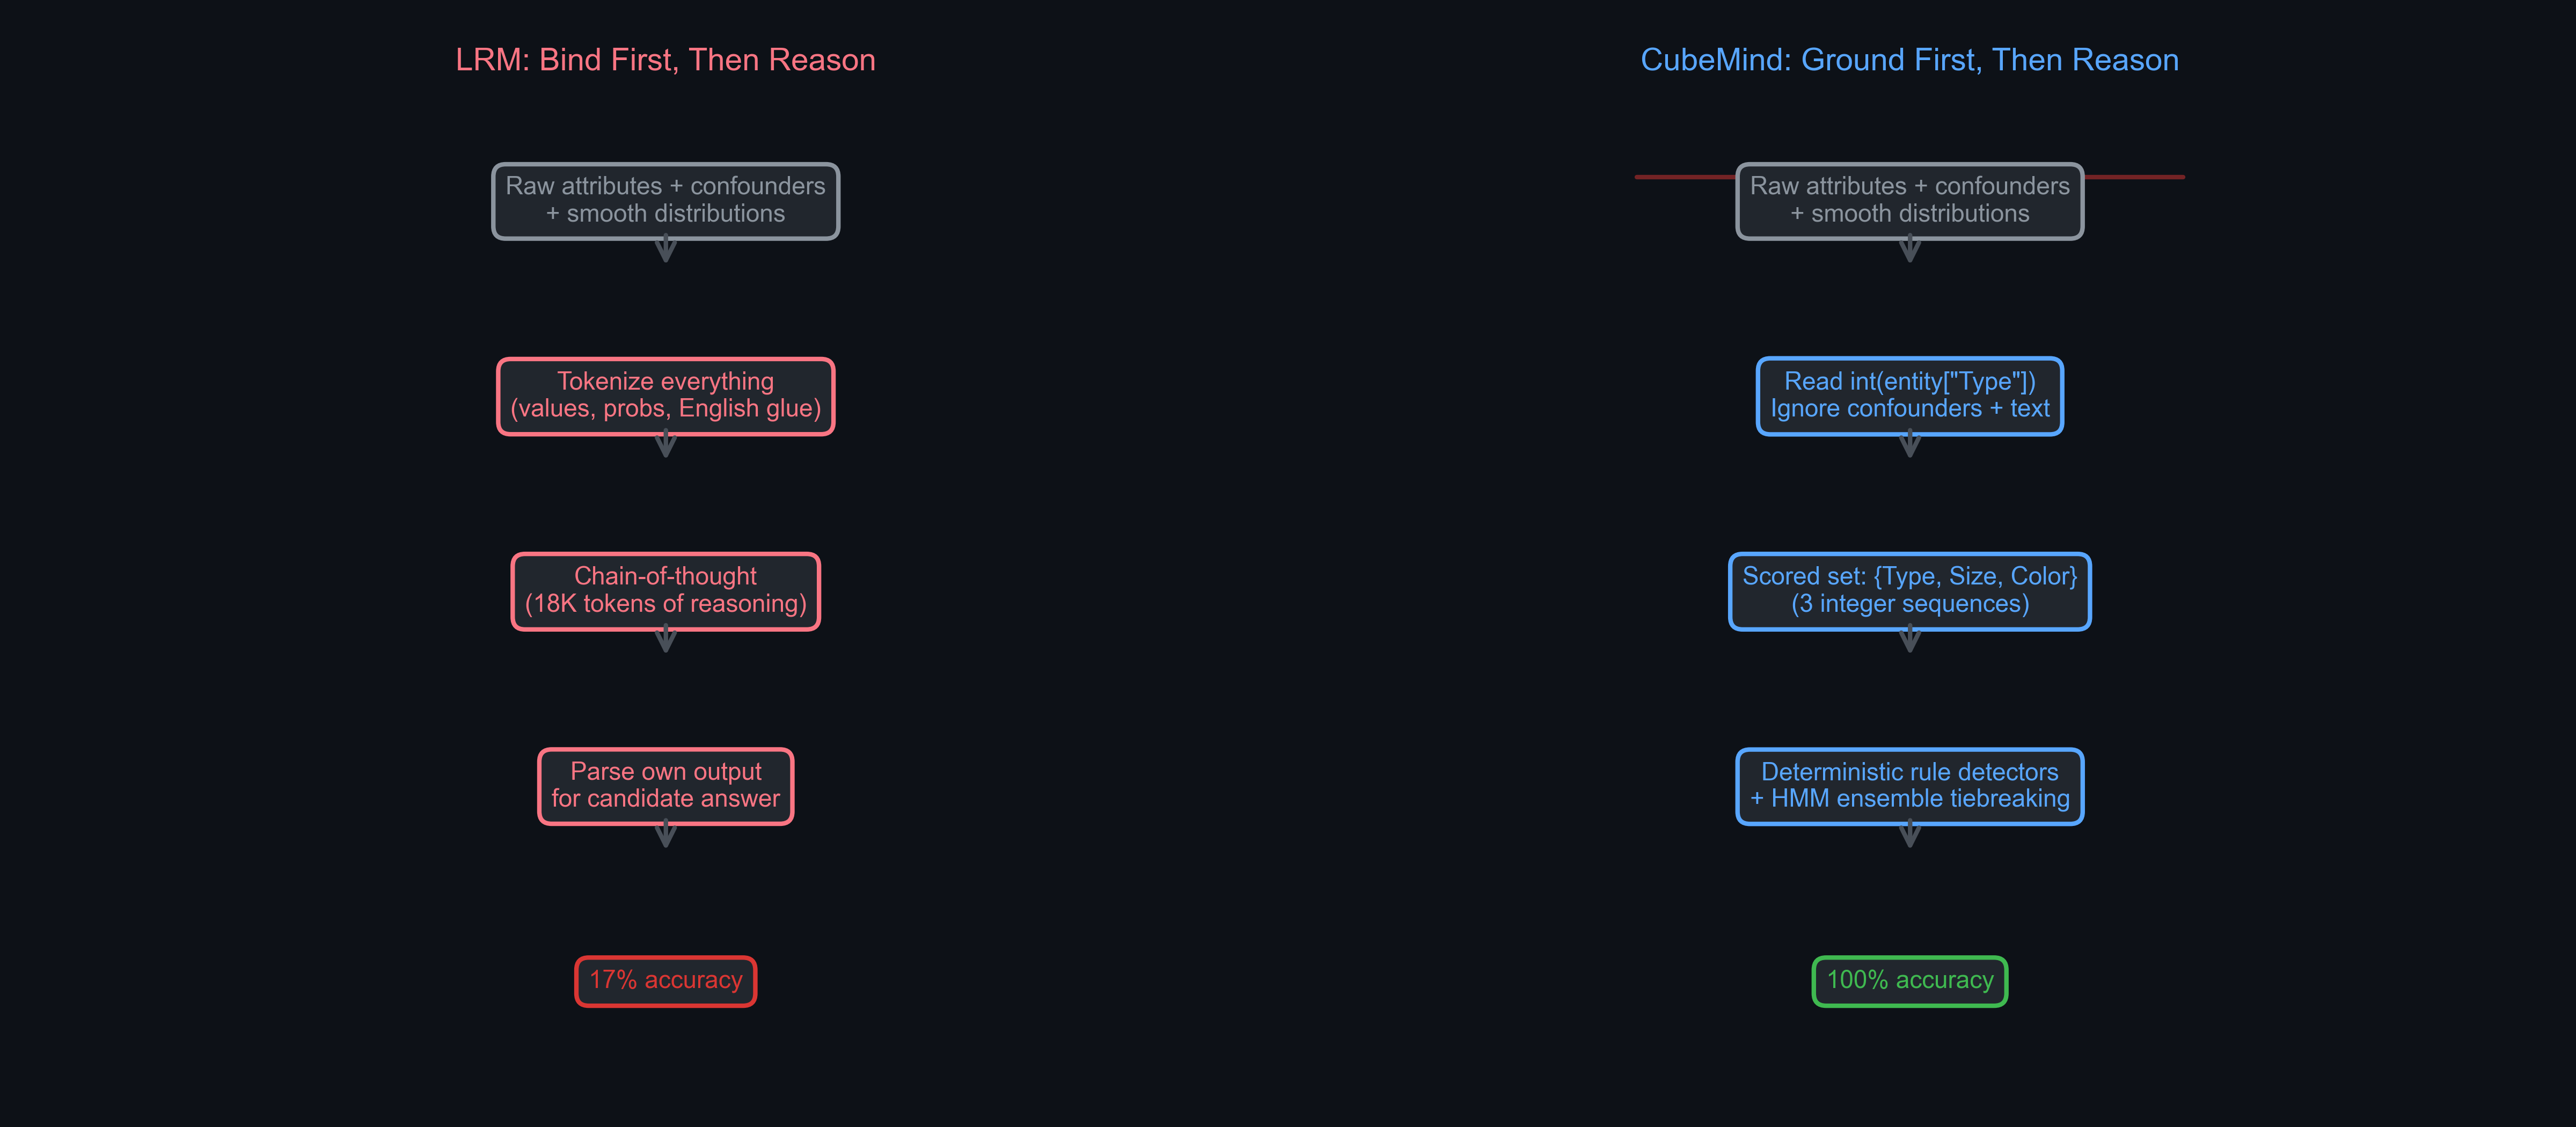
\includegraphics[width=\textwidth]{paper_fig6_double_binding.png}
    \caption{LRMs bind everything into tokens first, then reason. CubeMind grounds representations first, then applies deterministic reasoning.}
    \label{fig:double_binding}
\end{figure}

%----------------------------------------------------------------------
% References — placed after appendix so they don't interleave
%----------------------------------------------------------------------

\begin{thebibliography}{14}

\bibitem{raven1938}
J.~C.~Raven.
\newblock \emph{Progressive Matrices: A Perceptual Test of Intelligence}.
\newblock H.~K.~Lewis, London, 1938.

\bibitem{zhang2019raven}
C.~Zhang, F.~Gao, B.~Jia, Y.~Zhu, and S.-C.~Zhu.
\newblock {RAVEN}: A dataset for relational and analogical visual reasoning.
\newblock In \emph{CVPR}, 2019.

\bibitem{sicking2026iravenx}
J.~Sicking et~al.
\newblock {I-RAVEN-X}: A challenging out-of-distribution abstract visual reasoning benchmark.
\newblock \emph{arXiv:2510.17496}, 2026.

\bibitem{hersche2023nvsa}
M.~Hersche, M.~Zeqiri, L.~Benini, A.~Sebastian, and A.~Rahimi.
\newblock A neuro-vector-symbolic architecture for solving {Raven's} progressive matrices.
\newblock \emph{Nature Machine Intelligence}, 5:363--375, 2023.

\bibitem{friston2010free}
K.~Friston.
\newblock The free-energy principle: a unified brain theory?
\newblock \emph{Nature Reviews Neuroscience}, 11(2):127--138, 2010.

\bibitem{namjoshi2026active}
S.~V.~Namjoshi.
\newblock \emph{Fundamentals of Active Inference}.
\newblock 2026.

\bibitem{openai2025o3mini}
{OpenAI}.
\newblock o3-mini, 2025.

\bibitem{deepseek2025r1}
{DeepSeek}.
\newblock {DeepSeek-R1}, 2025.

\bibitem{huang2026reasoning}
F.~Huang.
\newblock Reasoning topology matters: Network-of-thought for complex reasoning tasks.
\newblock \emph{arXiv:2603.20730}, 2026.

\bibitem{neural_prediction2026}
Neural prediction errors as a unified cue for abstract visual reasoning.
\newblock \emph{IEEE TPAMI}, 2026.

\bibitem{resolve2026}
{RESOLVE}: Reasoning in hyperdimensional spaces with relational operations.
\newblock \emph{IEEE Access}, 2026.

\bibitem{world_models_robotics2023}
World models and predictive coding for cognitive and developmental robotics.
\newblock \emph{Taylor \& Francis}, 2023.

\bibitem{deep_active_inference2026}
Deep active inference agents for delayed and long-horizon environments.
\newblock \emph{OpenReview}, 2026.

\bibitem{graph_agreement2026}
Graph-theoretic agreement framework for multi-agent LLM systems.
\newblock \emph{UBOS}, 2026.

\end{thebibliography}

\end{document}
